\documentclass{article}%
\usepackage[T1]{fontenc}%
\usepackage[utf8]{inputenc}%
\usepackage{lmodern}%
\usepackage{textcomp}%
\usepackage{lastpage}%
\usepackage{geometry}%
\geometry{margin=1in}%
\usepackage{ragged2e}%
\usepackage{amsmath}%
\usepackage{graphicx}%
\usepackage{fancyhdr}%
%
\fancypagestyle{header}{%
\renewcommand{\headrulewidth}{0pt}%
\renewcommand{\footrulewidth}{0pt}%
\fancyhead{%
}%
\fancyfoot{%
}%
\fancyhead[L]{%
Report date: 9/14/2023%
\linebreak%
}%
\fancyhead[C]{%
Phius%
}%
\fancyhead[R]{%
Page \thepage\ of \pageref{LastPage}%
}%
}%
%
\begin{document}%
\normalsize%
\pagestyle{header}%
\begin{minipage}{\textwidth}%
\centering%
\begin{Large}%
\textbf{REVIVE 2024 Report}%
\end{Large}%
\linebreak%
\begin{large}%
Resilience and ADORB Summary%
\end{large}%
\linebreak%
\linebreak%
\begin{large}%
\textbf{Pizza Hut}%
\end{large}%
\end{minipage}%
\section{Introduction}%
\label{sec:Introduction}%
Some regular text and some%
\textit{italic text. }%
\newline%
Also some crazy characters: \$\&\#\{\}

%
\subsection{Math that is incorrect}%
\label{subsec:Maththatisincorrect}%
\[%
2*3 = 9%
\]

%
\section{Thermal Resilience}%
\label{sec:ThermalResilience}%
Some regular text and some

%
\subsection{Single Point Metrics}%
\label{subsec:SinglePointMetrics}%
\begin{tabular}{l|l|l}%
\hline%
Metric&Result&Unit\\%
\hline%
Heating SET Hours&56.4&°F hr\\%
Hours Below 2°C&2&hr\\%
\hline%
Caution (> 26.7, ≤ 32.2°C)&4&hr\\%
Extreme Caution (> 32.2, ≤ 39.4°C)&89&hr\\%
Danger (> 39.4, ≤ 51.7°C)&453&hr\\%
Extreme Danger (> 51.7°C)&858383&hr\\%
\hline%
Heating Battery Size&5&kWh\\%
Cooling Battery Size&6&kWh\\%
\hline%
\end{tabular}

%
\subsection{Graph Results}%
\label{subsec:GraphResults}%


\begin{figure}[h!]%
\centering%
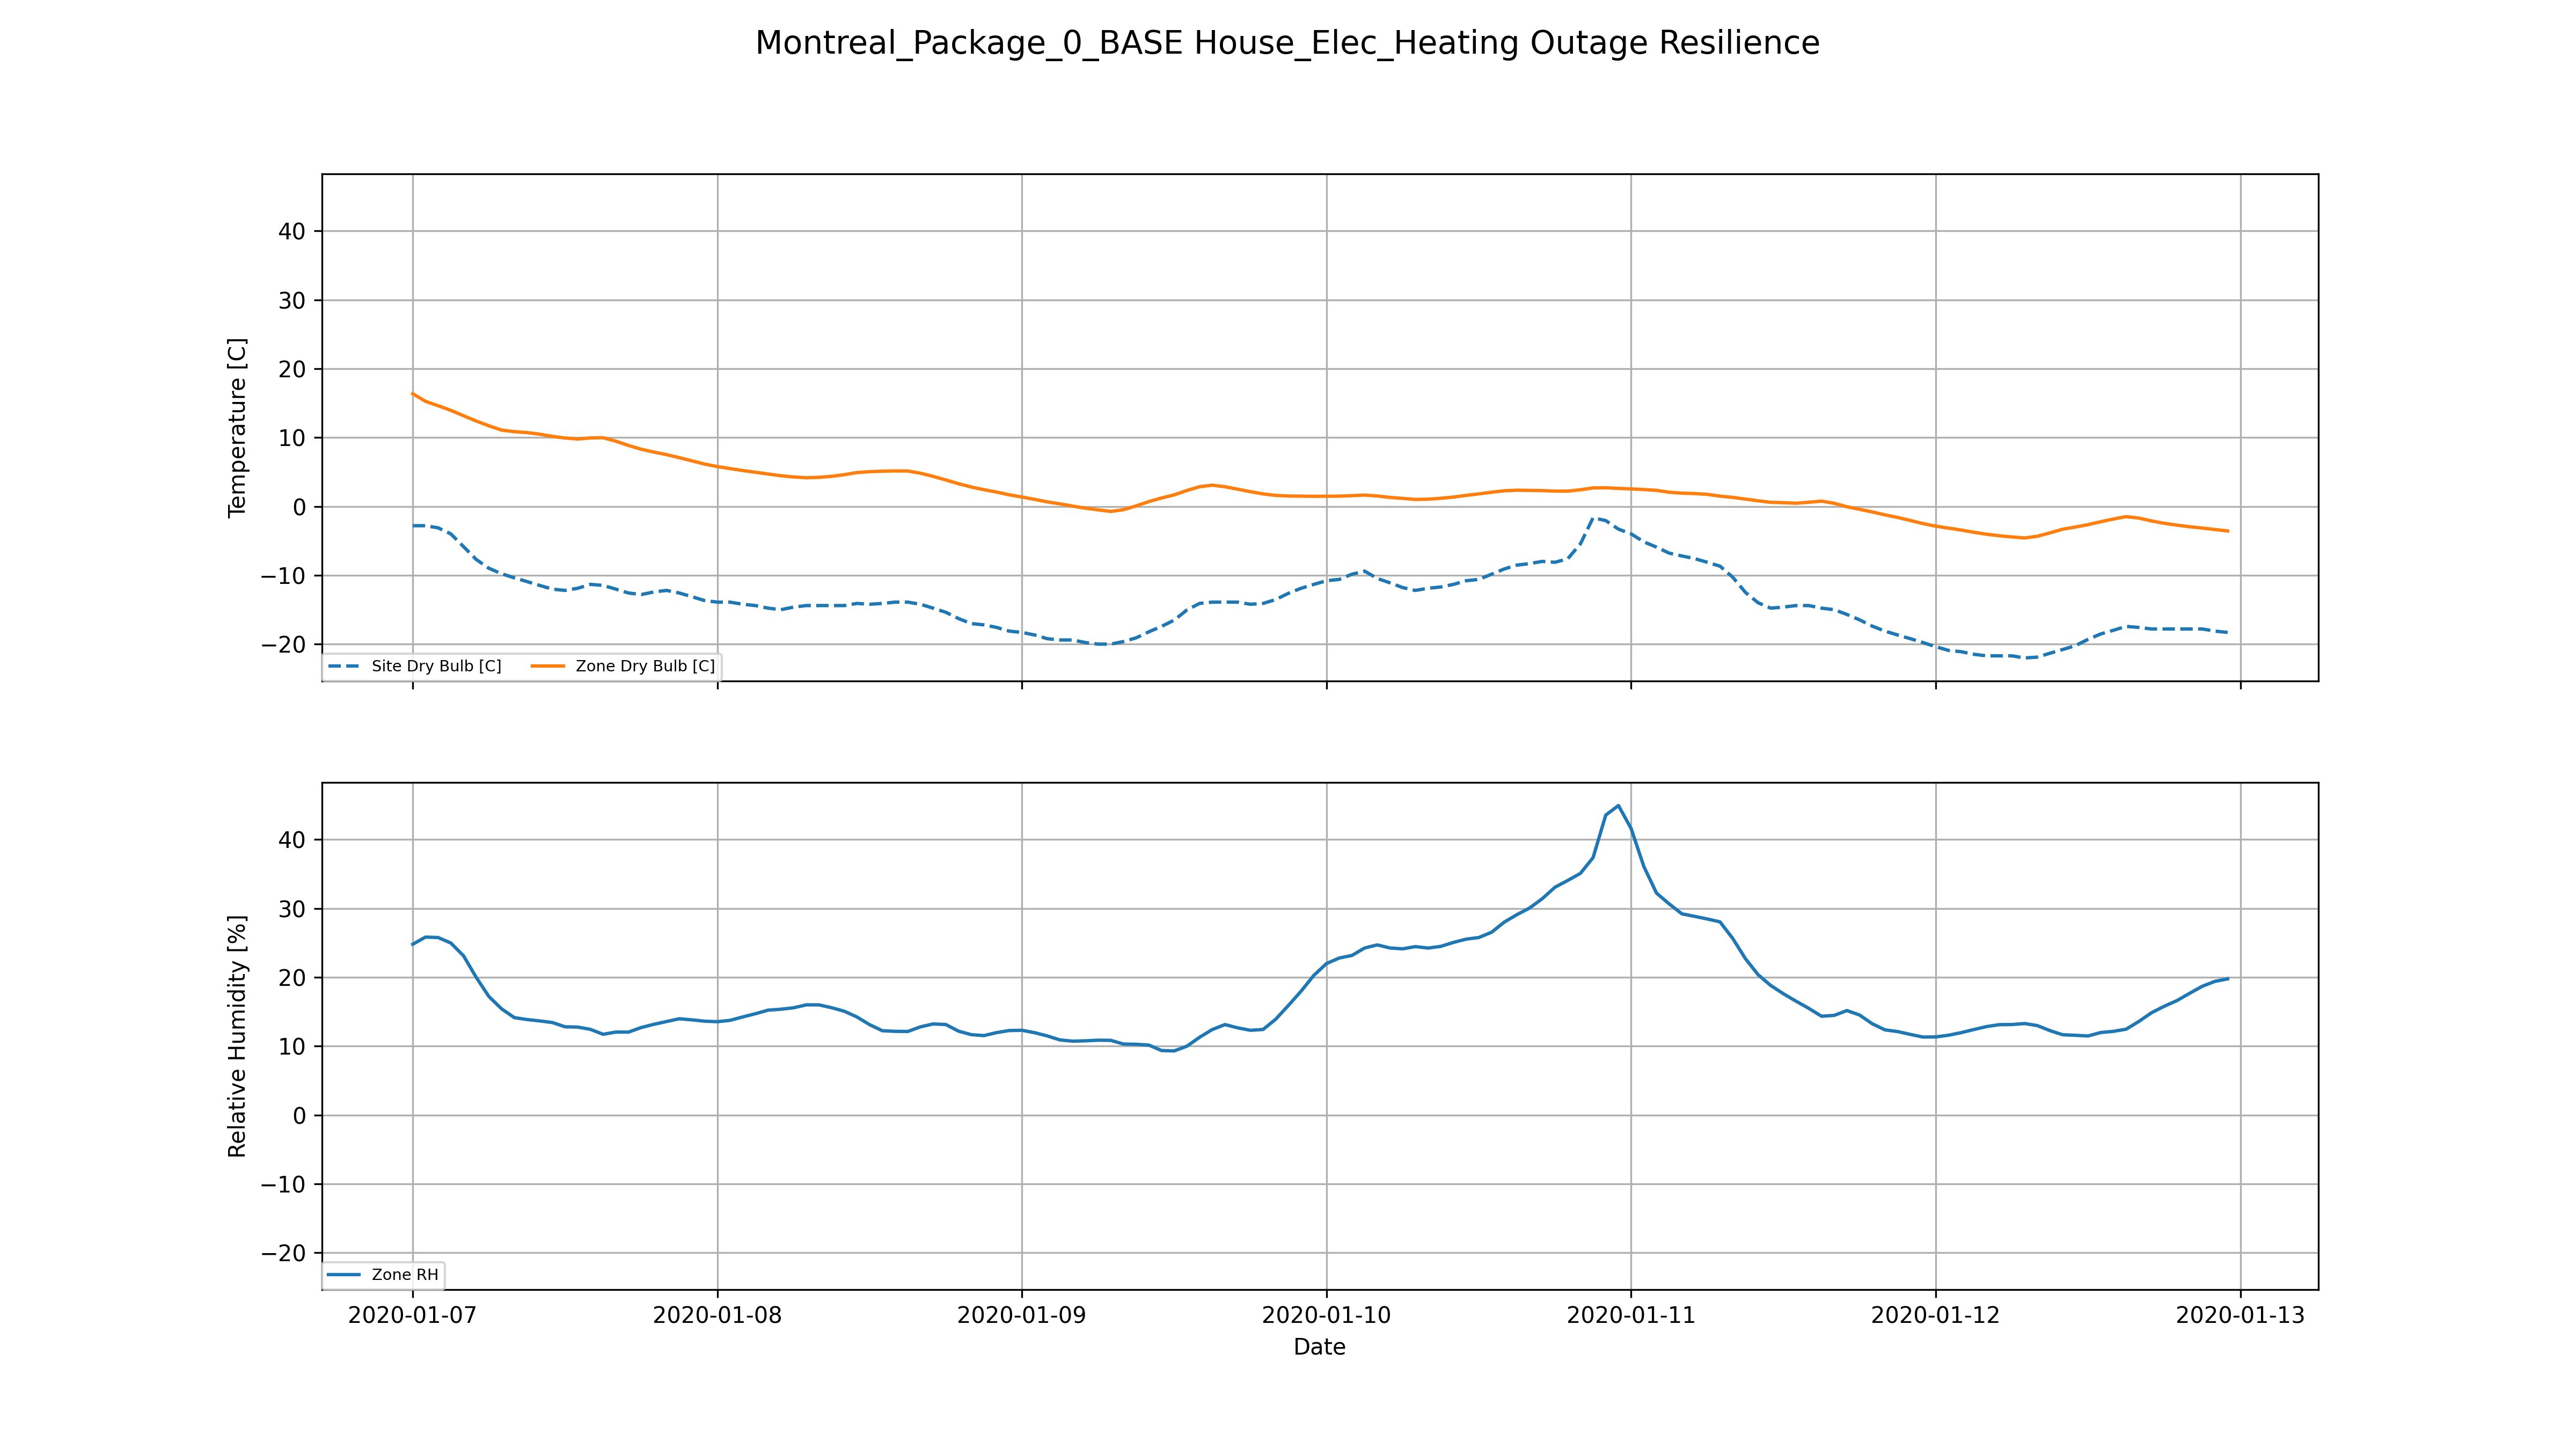
\includegraphics[width=6in]{C:/Users/amitc_crl/OneDrive/Documents/GitHub/REVIVE/REVIVE2024/Testing Files/Testing_2023-08-29/Name your batch of files_Montreal_Package_0_BASE House_Elec_Heating Outage Resilience Graphs.png}%
\end{figure}

%


\begin{figure}[h!]%
\centering%
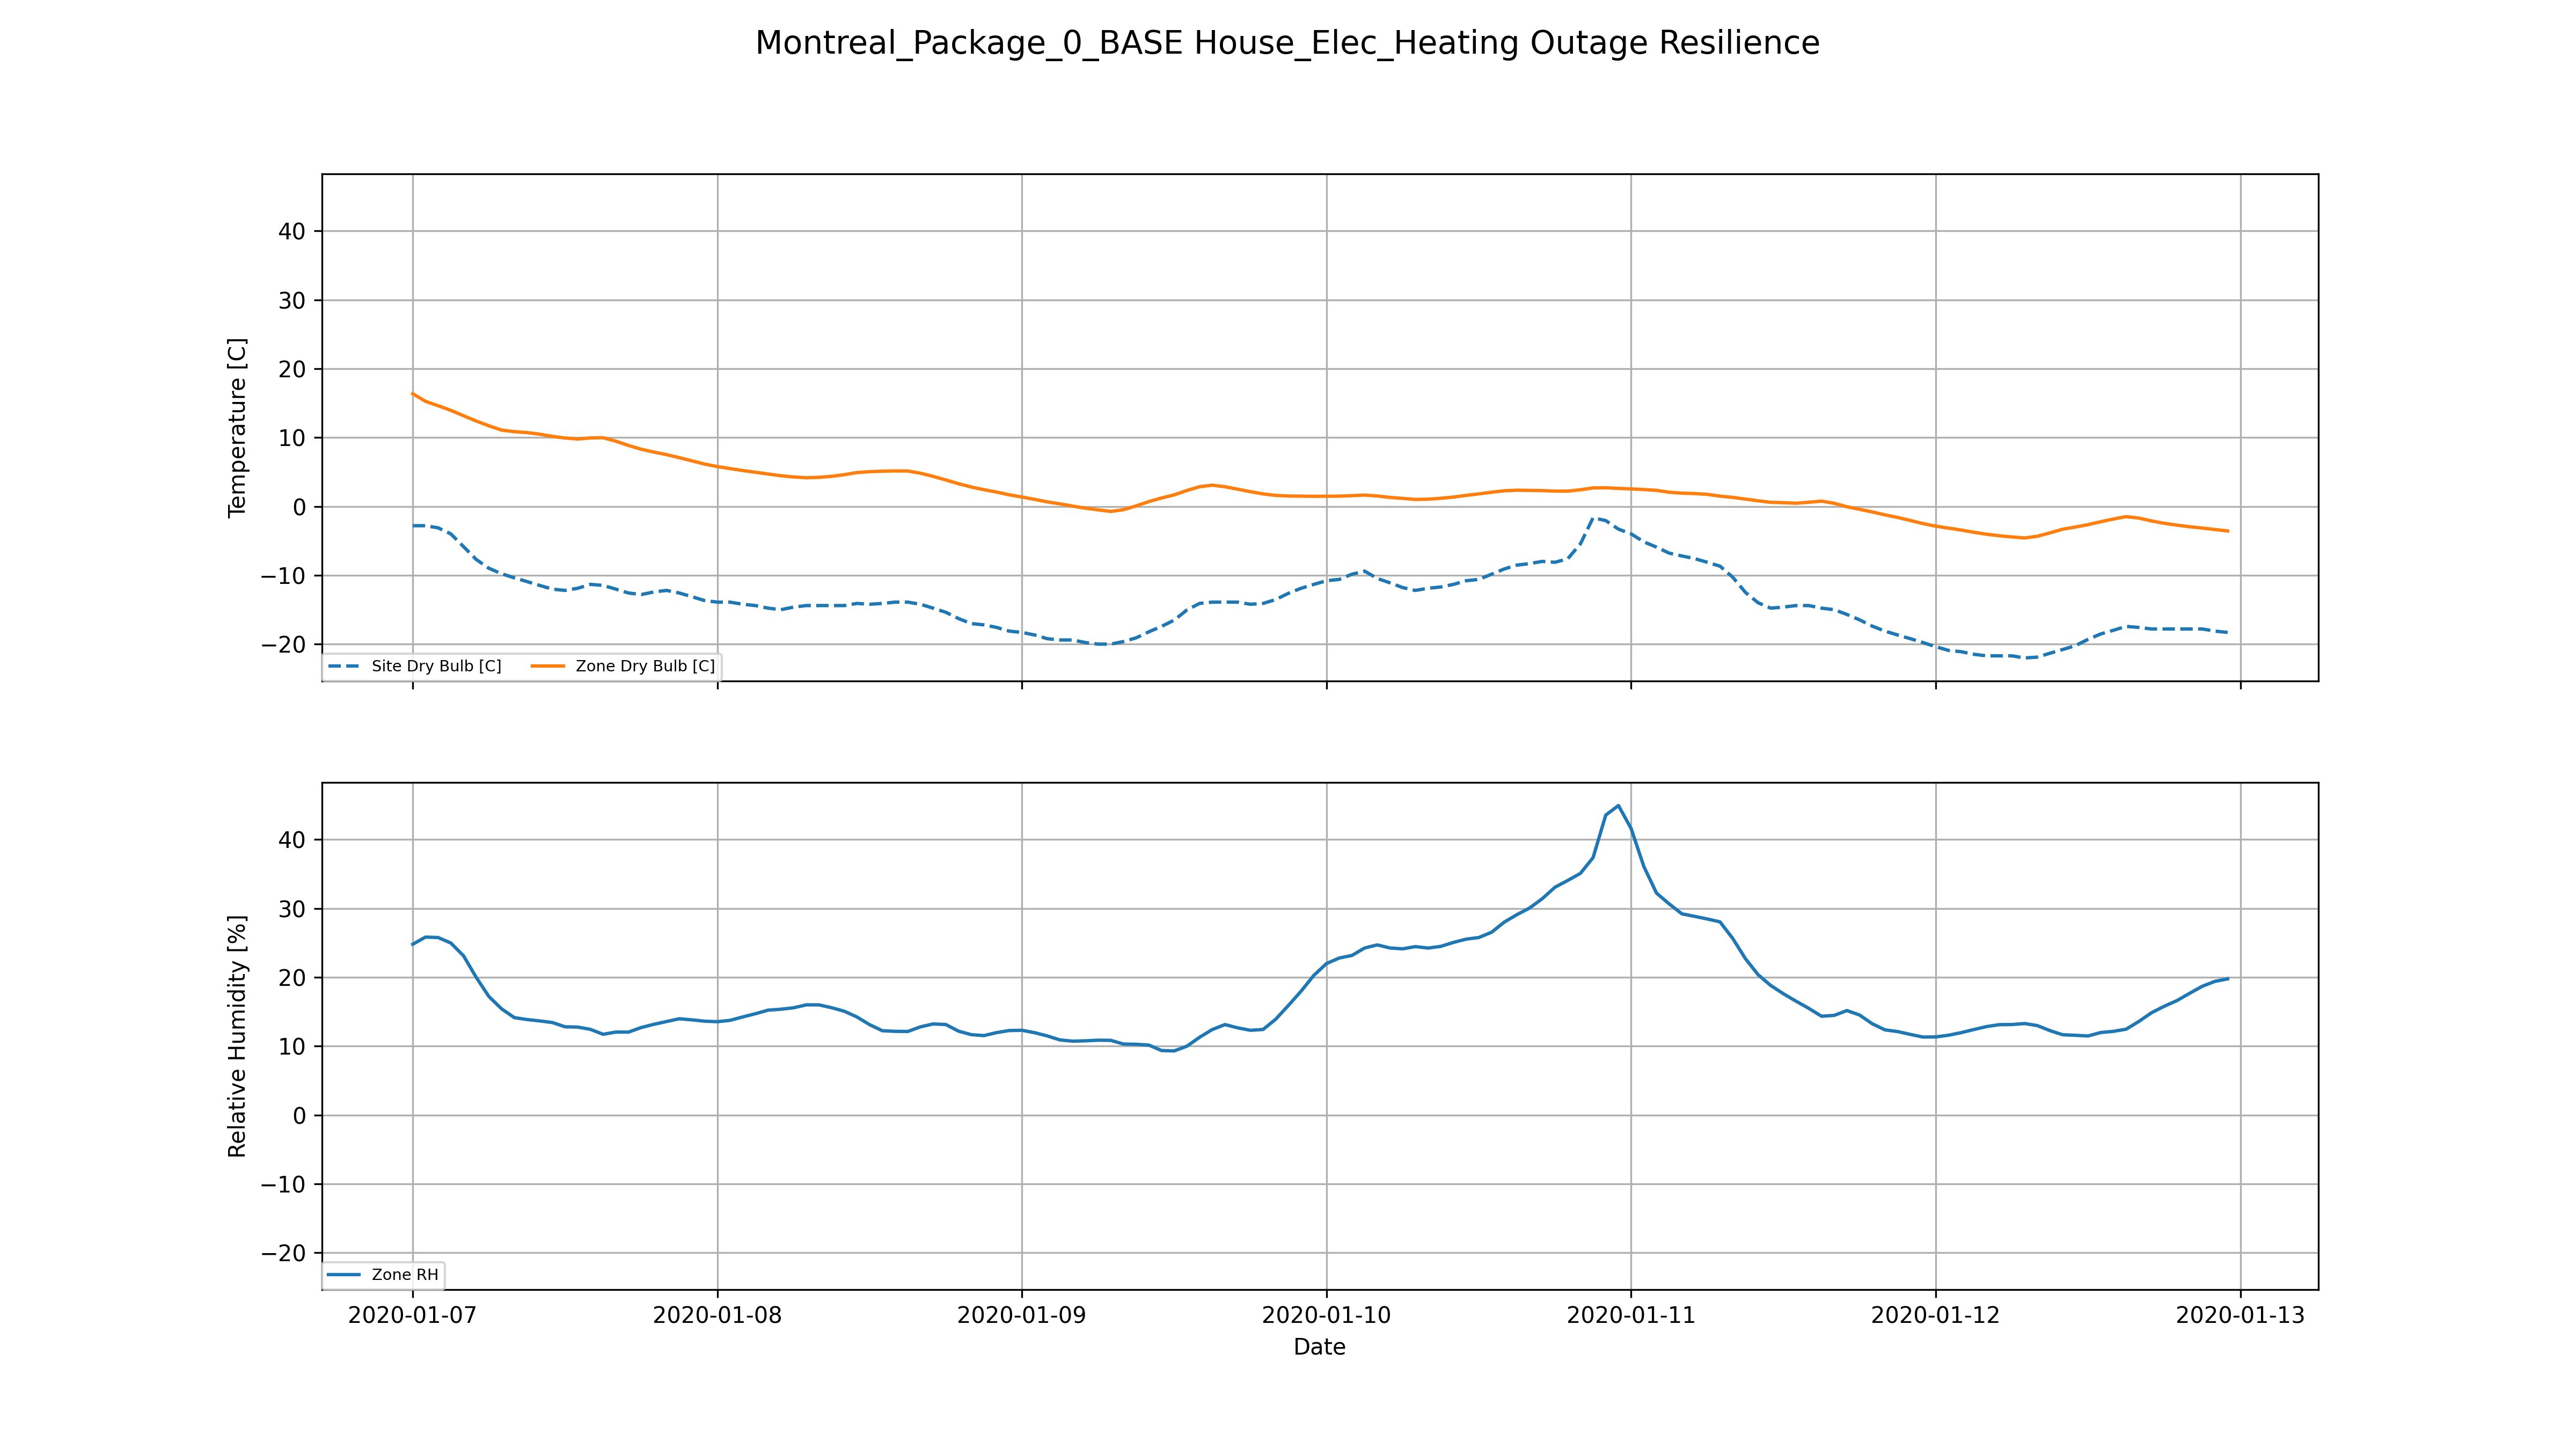
\includegraphics[width=6in]{C:/Users/amitc_crl/OneDrive/Documents/GitHub/REVIVE/REVIVE2024/Testing Files/Testing_2023-08-29/Name your batch of files_Montreal_Package_0_BASE House_Elec_Heating Outage Resilience Graphs.png}%
\end{figure}

%
\section{Annual and ADORB}%
\label{sec:AnnualandADORB}%
Some regular text and some

%
\subsection{Single Point Metrics}%
\label{subsec:SinglePointMetrics}%
\begin{tabular}{l|l|l}%
\hline%
Metric&Result&Unit\\%
\hline%
Energy Use Intensity&34.5&kBtu/ sf yr\\%
Peak Electrical Load&543&W\\%
\hline%
First Year Electric Cost&1505.02&\$\\%
First Cost&543254&\$\\%
Total ADORB Cost&572343&\$\\%
\hline%
\end{tabular}

%
\subsection{Graph Results}%
\label{subsec:GraphResults}%


\begin{figure}[h!]%
\centering%
\includegraphics[width=6in]{C:/Users/amitc_crl/OneDrive/Documents/GitHub/REVIVE/REVIVE2024/Testing Files/Testing_2023-08-29/Name your batch of files_Montreal_Package_3_IECC_Elec_ADORB_Wedge.png}%
\end{figure}

%


\begin{figure}[h!]%
\centering%
\includegraphics[width=6in]{C:/Users/amitc_crl/OneDrive/Documents/GitHub/REVIVE/REVIVE2024/Testing Files/Testing_2023-08-29/Name your batch of files_Montreal_Package_3B_IECC+0.04_Elec_ADORB_Bar.png}%
\end{figure}

%
\end{document}